%%% Преамбула %%%
\documentclass[a4paper,14pt]{extarticle}

\usepackage{fontspec} % XeTeX
\usepackage{xunicode} % Unicode для XeTeX
\usepackage{xltxtra}  % Верхние и нижние индексы
\usepackage{pdfpages} % Вставка PDF
\usepackage[outputdir=aux]{minted}   % Вставка и подсветка кода
\usemintedstyle{xcode}

\usepackage{listings} % Оформление исходного кода
\lstset{
    basicstyle=\small\ttfamily, % Размер и тип шрифта
    breaklines=true,            % Перенос строк
    tabsize=2,                  % Размер табуляции
    frame=single,               % Рамка
    literate={--}{{-{}-}}2,     % Корректно отображать двойной дефис
    literate={---}{{-{}-{}-}}3  % Корректно отображать тройной дефис
}

% Шрифты, xelatex
\defaultfontfeatures{Ligatures=TeX}
\setmainfont{Times New Roman} % Нормоконтроллеры хотят именно его
\newfontfamily{\cyrillicfont}{Times New Roman}
% \setsansfont{Liberation Sans} % Тут я его не использую, но если пригодится
\setmonofont{Courier New} % Моноширинный шрифт для оформления кода
\newfontfamily{\cyrillicfonttt}{Courier New}

% Формулы
\usepackage{mathtools,unicode-math} % Не совместим с amsmath
\setmathfont{XITS Math}             % Шрифт для формул: https://github.com/khaledhosny/xits-math
\numberwithin{equation}{section}    % Формула вида секция.номер

% Русский язык
\usepackage{polyglossia}
\setdefaultlanguage{russian}

% Абзацы и списки
\usepackage{enumerate}   % Тонкая настройка списков
\usepackage{indentfirst} % Красная строка после заголовка
\usepackage{float}       % Расширенное управление плавающими объектами
\usepackage{multirow}    % Сложные таблицы

% Пути к каталогам с изображениями
\usepackage{graphicx} % Вставка картинок и дополнений
\graphicspath{{images/}}

% Формат подрисуночных записей
\usepackage{chngcntr}

% Сбрасываем счетчик таблиц и рисунков в каждой новой главе
\counterwithin{figure}{section}
\counterwithin{table}{section}

% Гиперссылки
\usepackage{hyperref}
\hypersetup{
    colorlinks, urlcolor={black}, % Все ссылки черного цвета, кликабельные
    linkcolor={black}, citecolor={black}, filecolor={black},
    pdfauthor={Амет Умеров},
    pdftitle={Исследование процессов обеспечения безопасности облачных сред}
}

% Оформление библиографии и подрисуночных записей через точку
\makeatletter
\renewcommand*{\@biblabel}[1]{\hfill#1.}
\renewcommand*\l@section{\@dottedtocline{1}{1em}{1em}}
\renewcommand{\thefigure}{\thesection.\arabic{figure}} % Формат рисунка секция.номер
\renewcommand{\thetable}{\thesection.\arabic{table}}   % Формат таблицы секция.номер
\def\redeflsection{\def\l@section{\@dottedtocline{1}{0em}{10em}}}
\makeatother

\renewcommand{\baselinestretch}{1.4} % Полуторный межстрочный интервал
\parindent 1.27cm % Абзацный отступ

\sloppy             % Избавляемся от переполнений
\hyphenpenalty=1000 % Частота переносов
\clubpenalty=10000  % Запрещаем разрыв страницы после первой строки абзаца
\widowpenalty=10000 % Запрещаем разрыв страницы после последней строки абзаца

% Отступы у страниц
\usepackage{geometry}
\geometry{left=2cm}
\geometry{right=2cm}
\geometry{top=2cm}
\geometry{bottom=2cm}

% Списки
\usepackage{enumitem}
\setlist[enumerate,itemize]{leftmargin=12.7mm} % Отступы в списках

\makeatletter
    \AddEnumerateCounter{\asbuk}{\@asbuk}{м)}
\makeatother
\setlist{nolistsep}                           % Нет отступов между пунктами списка
\renewcommand{\labelitemi}{--}                % Маркер списка --
\renewcommand{\labelenumi}{\asbuk{enumi})}    % Список второго уровня
\renewcommand{\labelenumii}{\arabic{enumii})} % Список третьего уровня

% Содержание
\usepackage{tocloft}
\renewcommand{\cfttoctitlefont}{\hspace{0.38\textwidth}\MakeTextUppercase} % СОДЕРЖАНИЕ
\renewcommand{\cftsecfont}{\hspace{0pt}}            % Имена секций в содержании не жирным шрифтом
\renewcommand\cftsecleader{\cftdotfill{\cftdotsep}} % Точки для секций в содержании
\renewcommand\cftsecpagefont{\mdseries}             % Номера страниц не жирные
\setcounter{tocdepth}{3}                            % Глубина оглавления, до subsubsection

% Список иллюстративного материала
\renewcommand{\cftloftitlefont}{\hspace{0.17\textwidth}\MakeTextUppercase}
\renewcommand{\cftfigfont}{Рисунок }
\addto\captionsrussian{\renewcommand\listfigurename{Список иллюстративного материала}}

% Список табличного материала
\renewcommand{\cftlottitlefont}{\hspace{0.2\textwidth}\MakeTextUppercase}
\renewcommand{\cfttabfont}{Таблица }
\addto\captionsrussian{\renewcommand\listtablename{Список табличного материала}}

% Нумерация страниц посередине сверху
\usepackage{fancyhdr}
\pagestyle{fancy}
\fancyhf{}
\cfoot{\textrm{\thepage}}
\fancyheadoffset{0mm}
\fancyfootoffset{0mm}
\setlength{\headheight}{17pt}
\renewcommand{\headrulewidth}{0pt}
\renewcommand{\footrulewidth}{0pt}
\fancypagestyle{plain}{
    \fancyhf{}
    \cfoot{\textrm{\thepage}}
}

% Формат подрисуночных надписей
\RequirePackage{caption}
\DeclareCaptionLabelSeparator{defffis}{ -- } % Разделитель
\captionsetup[figure]{justification=centering, labelsep=defffis, format=plain} % Подпись рисунка по центру
\captionsetup[table]{justification=raggedright, labelsep=defffis, format=plain, singlelinecheck=false} % Подпись таблицы слева
\addto\captionsrussian{\renewcommand{\figurename}{Рисунок}} % Имя фигуры

% Пользовательские функции
\newcommand{\addimg}[4]{ % Добавление одного рисунка
    \begin{figure}
        \centering
        \includegraphics[width=#2\linewidth]{#1}
        \caption{#3} \label{#4}
    \end{figure}
}
\newcommand{\addimghere}[4]{ % Добавить рисунок непосредственно в это место
    \begin{figure}[H]
        \centering
        \includegraphics[width=#2\linewidth]{#1}
        \caption{#3} \label{#4}
    \end{figure}
}
\newcommand{\addtwoimghere}[5]{ % Вставка двух рисунков
    \begin{figure}[H]
        \centering
        \includegraphics[width=#2\linewidth]{#1}
        \hfill
        \includegraphics[width=#3\linewidth]{#2}
        \caption{#4} \label{#5}
    \end{figure}
}

% Заголовки секций в оглавлении в верхнем регистре
\usepackage{textcase}
\makeatletter
\let\oldcontentsline\contentsline
\def\contentsline#1#2{
    \expandafter\ifx\csname l@#1\endcsname\l@section
        \expandafter\@firstoftwo
    \else
        \expandafter\@secondoftwo
    \fi
    {\oldcontentsline{#1}{\MakeTextUppercase{#2}}}
    {\oldcontentsline{#1}{#2}}
}
\makeatother

% Оформление заголовков
\usepackage[compact,explicit]{titlesec}
\titleformat{\section}{}{}{12.5mm}{\centering{\thesection\quad\MakeTextUppercase{#1}}\vspace{1.5em}}
\titleformat{\subsection}[block]{\vspace{1em}}{}{12.5mm}{\thesubsection\quad#1\vspace{1em}}
\titleformat{\subsubsection}[block]{\vspace{1em}\normalsize}{}{12.5mm}{\thesubsubsection\quad#1\vspace{1em}}
\titleformat{\paragraph}[block]{\normalsize}{}{12.5mm}{\MakeTextUppercase{#1}}

% Секции без номеров (введение, заключение...), вместо section*{}
\newcommand{\anonsection}[1]{
    \phantomsection % Корректный переход по ссылкам в содержании
    \paragraph{\centerline{{#1}}\vspace{1em}}
    \addcontentsline{toc}{section}{#1}
}

% Секция для аннотации (она не включается в содержание)
\newcommand{\annotation}[1]{
    \paragraph{\centerline{{#1}}\vspace{1em}}
}

% Секция для списка иллюстративного материала
\newcommand{\lof}{
    \phantomsection
    \listoffigures
    \addcontentsline{toc}{section}{\listfigurename}
}

% Секция для списка табличного материала
\newcommand{\lot}{
    \phantomsection
    \listoftables
    \addcontentsline{toc}{section}{\listtablename}
}

% Секции для приложений
\newcommand{\appsection}[1]{
    \phantomsection
    \paragraph{\centerline{{#1}}}
    \addcontentsline{toc}{section}{{#1}}
}

% Библиография: отступы и межстрочный интервал
\makeatletter
\renewenvironment{thebibliography}[1]
    {\section*{\refname}
        \list{\@biblabel{\@arabic\c@enumiv}}
           {\settowidth\labelwidth{\@biblabel{#1}}
            \leftmargin\labelsep
            \itemindent 16.7mm
            \@openbib@code
            \usecounter{enumiv}
            \let\p@enumiv\@empty
            \renewcommand\theenumiv{\@arabic\c@enumiv}
        }
        \setlength{\itemsep}{0pt}
    }
\makeatother

\usepackage{lastpage} % Подсчет количества страниц
\setcounter{page}{3}  % Начало нумерации страниц

\title{Разработка распределенной системы обработки видео}
\author{Евгений Щибриков}

\begin{document}

\tableofcontents

\newpage

\section{Введение}

\subsection{Проблема производства видеоконтента с людьми}

Большая проблема при производстве видеоконтента в рекламе с других областях заключается в привязке к конкретному человеку. Используя конкретного человека, а особенно знаменитость, например, в рекламе, компании имеют дело с постоянными рисками и неудобствами. Это увеличивающиеся расходы (человек становиться более известным и "растет в цене"), сложности в планировании сьемок, опоздания и подобные проблемы.

Этих проблем можно избежать если не привязываться к конкретному физическому человеку. Можно снимать видео с виртуальным персонажем, созданным с помощью компьютерной графики, или купить права на использование изображения человека, и монтировать контент, накладывая лицо на актера. Таким образом можно взять любого актера и сделать его таким, каким привык его видеть зритель.

Нужно понимать, что подобный монтаж с помощью компьютерной графики является очень сложным и дорогим. Хотя это и позволяет избежать многих рисков связанных с человеческим фактором, производство может обходиться не дешевле, чем сьемки знаменитости.

Но с последними исследованиями в области нейронных сетей оказалось, что и эту проблему можно решить. Современные модели позволяют накладывать лицо на актера на видео автоматически, без ручного труда дизайнеров и специалистов по видеомонтажу. Ранние решения для этой цели требовали специального обучения модели для конкретной пары актера и лица, а так же обширный набор данных, включающий сьемки головы с разных ракурсов и с разными выражениями лица. Более того, требовалась ручная доработка результата, чтобы считать его удовлетворительным. Самые последние решения дают возможность замены лица по одному снимку и получение результата, не требующего доработок.

\section{Предлагаемое решение}

В этой работе рассматривается разработка распределенной многопользовательской системы для наложения лица на видео.

Такая система позволит пользователям за определенную плату получать достаточно качественное наложение лиц без каких-либо требований к навыкам разработки или использования нейронных моделей. 

Процесс наложения лиц достаточно дорогой и требует дорогостоящей инфраструктуры в серверов с графическими процессорами. Поэтому система не может быть бесплатной и должна быть ориентирована на платежеспособных пользователей. Исходя из этого для разработки и продвижения сервиса предлагается стратегия b2b, т.е. позиционирование на бизнес-пользователей, работающих в области создания аудиовизуального контента, например маркетинговые агенства.

\section{Постановка задачи}

Разработать систему, позволяющую неограниченному количеству пользователей обрабатывать видеоконтент с целью наложения некоторого лица персонажа (реального или виртуального) на лицо актера не видео. Системой должен иметь возможность воспользоваться любой человек, без особенной технической подготовки.

Система должна поддерживать масштабирование для неограниченного числа пользователей.

Так как обработка видео может занимать продолжительное время, то должна быть возможность параллельной обработки на нескольких серверах с целью ускорения.

Система должна иметь пользовательский интерфейс в виде веб-приложения, доступный в интернете.

\subsection{Начальные ограничения}

Основой системы служит ансамбль нейронных сетей, комбинирующий сети для сегментации лица, замены лица (identity injection) и сеть для повышения качества изображения (super resolution).

В данной работе не рассматриваются технические детали этого решения, вместо этого основным продуктом является программный комплекс, построенный на его основе.

Основными ограничениями данного ансамбля является скорость работы и высокие требования к аппаратному обеспечению.

\section{Описание методов решения}

\subsection{Клиент-серверная архитектура фронтенда}

Для разработки внешней части приложения выбрана клиент-серверная архитектура.

Выполнение вычислительно сложных операций, необходимых для решения задачи, возможно на клиентских устройствах в очень ограниченном объеме и несет множество проблем, таких как необходимость держать устройство включенным, потеря

Такое решение позволяет производить вычислительно сложные операции на серверах, так же сохраняя там приватную информацию о системе.

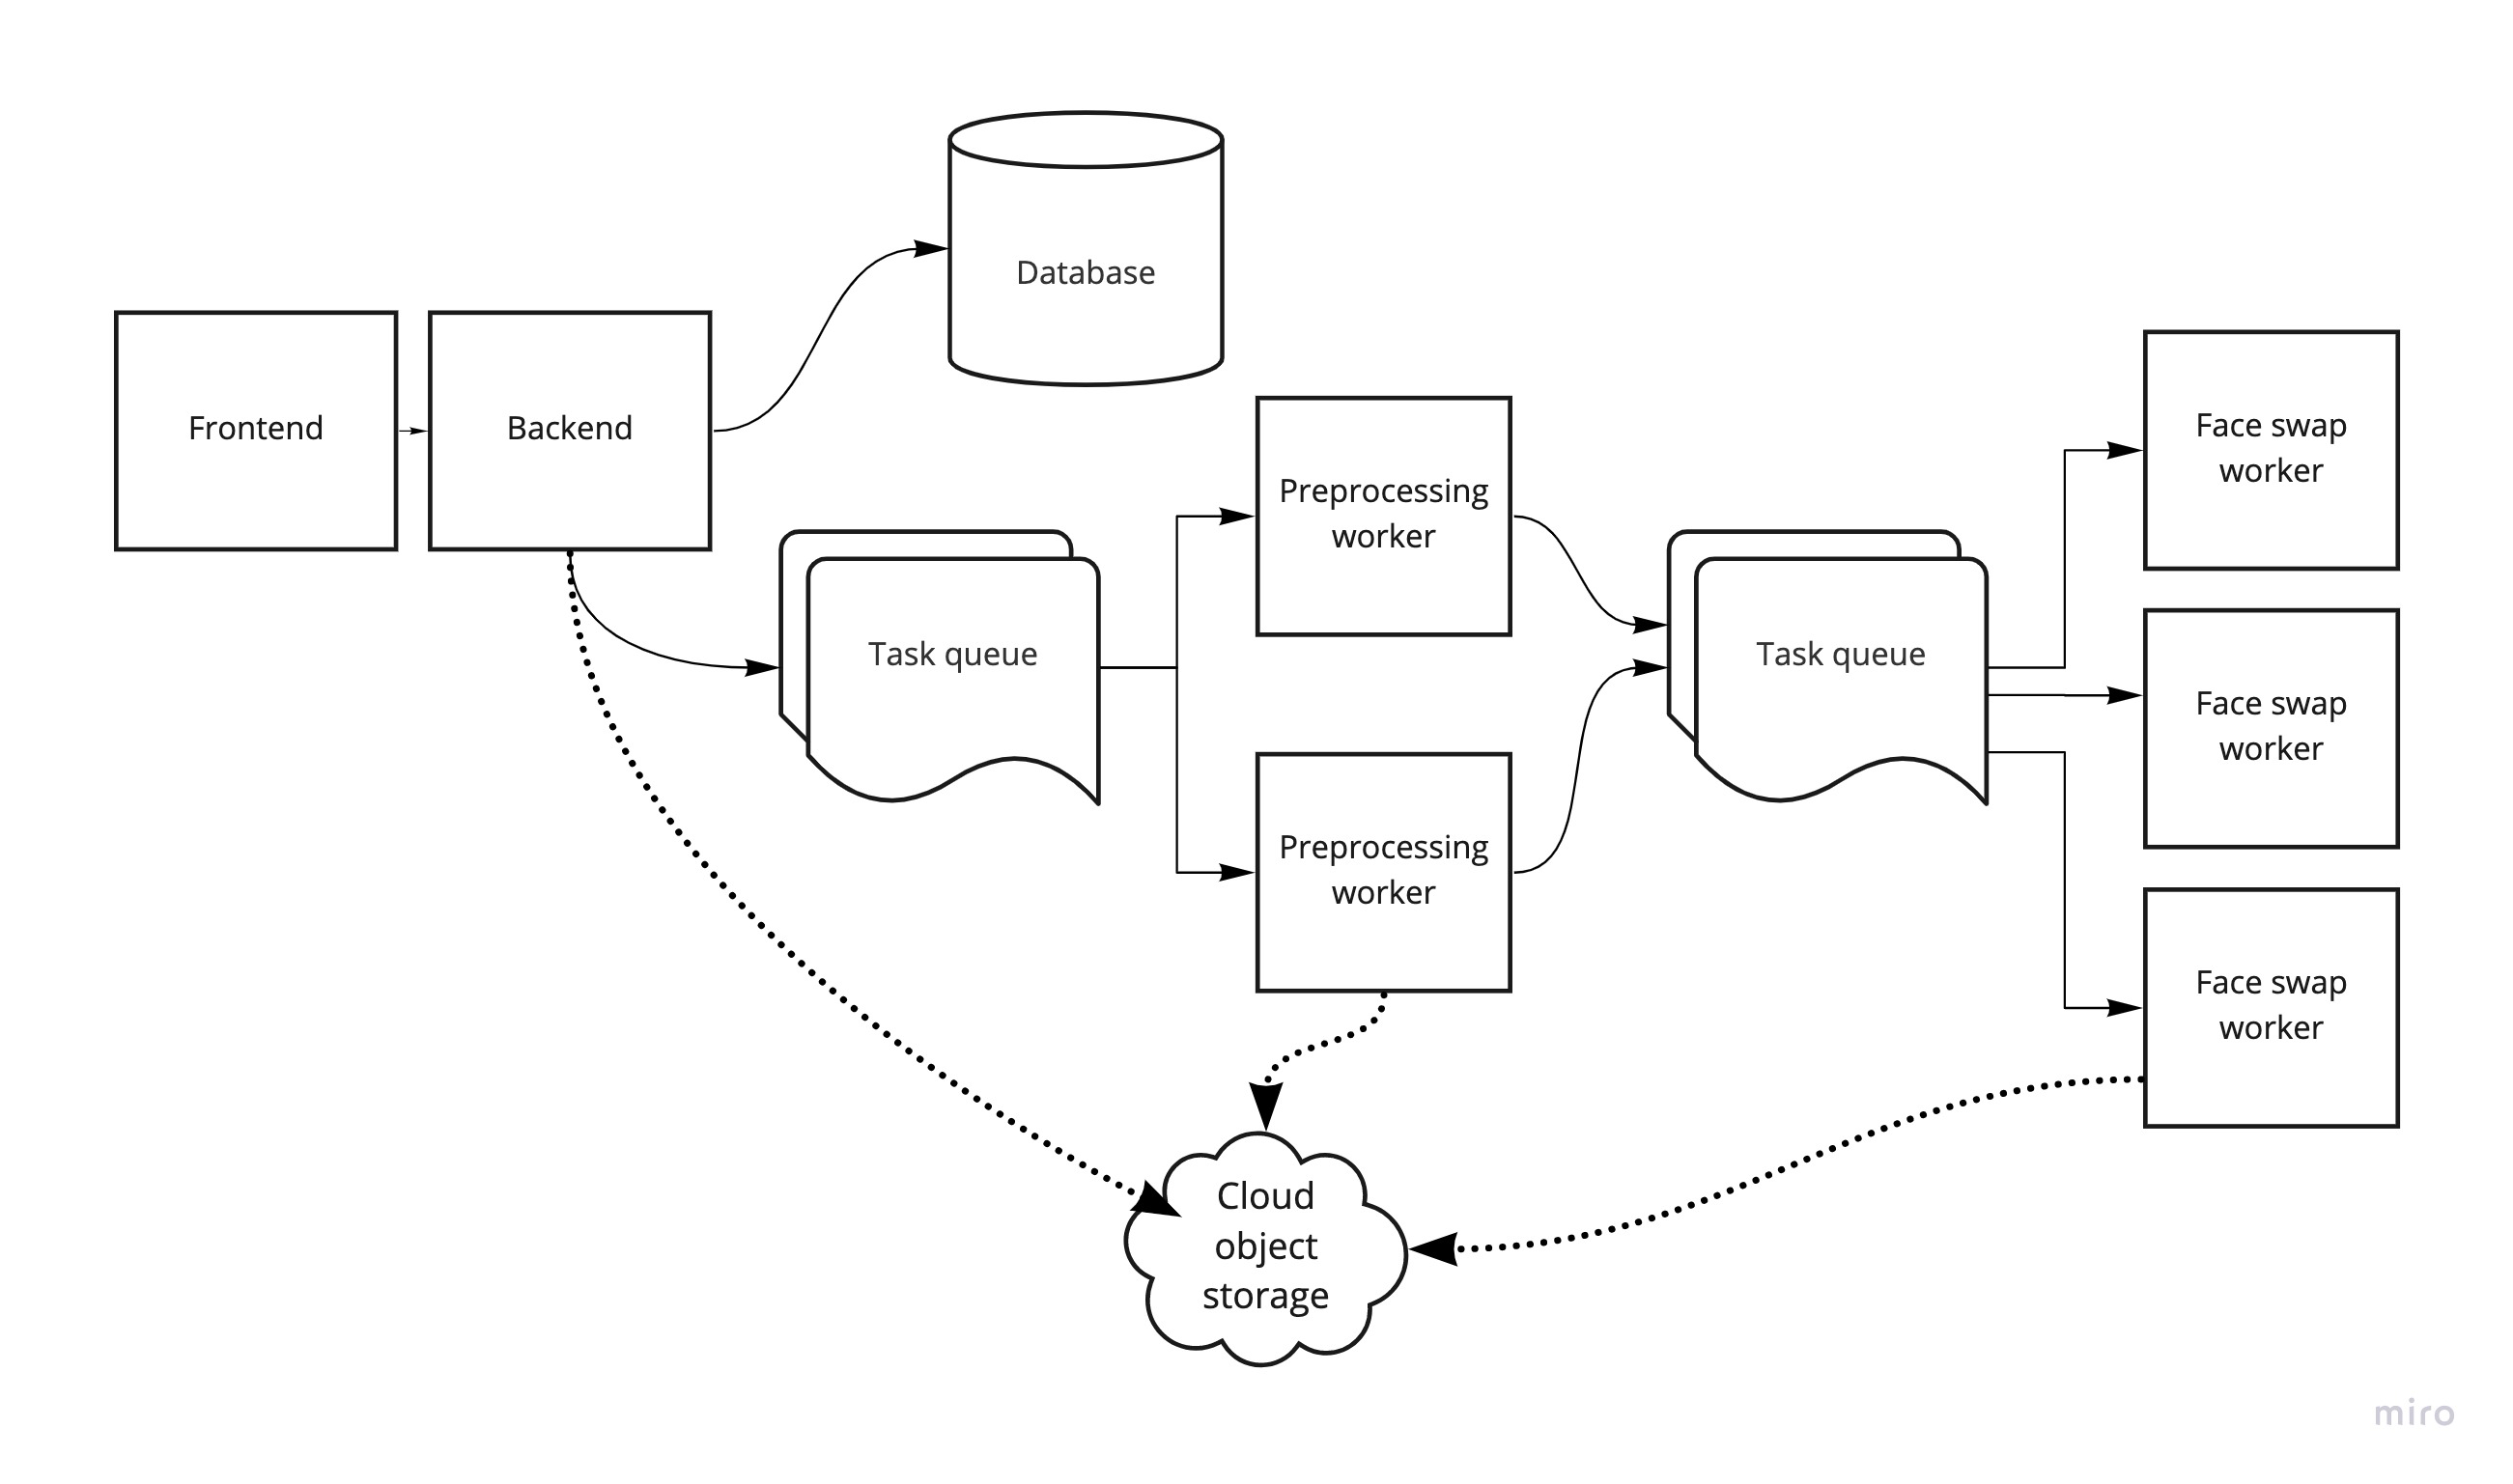
\includegraphics[width=\textwidth]{malivar_service_architecture}

\subsection{Инфраструктура}

В любой системе центральным вопросом инфраструктуры является расположение серверов. Под разработкой обычно подразумевается создание программного продукта, но когда дело касается разворачивания приложения в публичный доступ, возникает вопрос - покупать и располагать физические сервера у себя в компании или дата-центре или воспользоваться облачными провайдерами и получать необходимые мощности по подписке.

Рассмотрим некоторые особенности обоих вариантов.

Собственные сервера приобретаются один раз и могут стоить достаточно дешево, в сравнении с ежемесячными счетами от облачного провайдера. На первый взгляд из постоянных расходов они требуют лишь электричество и интернет. Но в деталях ситуация оказывается гораздо сложнее.

Собственные сервера требуют настройки и постоянного обслуживания, пример - обновления ПО. Для того, чтобы обеспечить непрерывную работы потребуются резервные интернет-каналы, запасной источник питания (например, ИБП).
Так же сервера отличаются от обычных компьютеров тем - они ориентированы на постоянную работу и имеют свои особенности. Например, шум и необходимость серьезного охлаждения. Обычно это проявляются в том, что для содержания своих серверов выделяют отдельную комнату - серверную.

Помимо собственно поддержки самого аппаратного обеспечения и операционных систем серверов, собственные сервера лишают возможности использования дополнительных услуг облачных провайдеров - управляемые (managed) сервисы, автоматическая репликация, в том числе геораспредленная, управление доступом и многое другое.

Если учитывать своимость обслуживания, собственные сервера могут оказаться гораздо дороже облачных услуг.

Облачные провайдеры, напротив, предоствляют максимально удобные, готовые и самоподдерживаемые сервисы, особенно при использовании не чистых виртуальных машин, а готовых сервисов, таких как управляемые базы данных, управляемый Kubernetes, файловое хранилище. Облачные провайдеры предоствляют автоматическое резервное копирование и обновление. Серьезным минусов использования "облаков" является так называемый vendor-lock - завязка на конкретного провайдера и невозможность (или очень высокая стоимость) переноса инфраструктуры от него. Это случается, если на проекте активно используются уникальные услуги, не предоставляемые или сильно отличающиеся у других провайдеров.

Для данного проекта было выбрано использования облачного провайдера Azure для размещения инфраструктуры. Это сервис от компании Microsoft. Он содержит огромное количество готовых сервисов и удобный веб-интерфейс для управления инфраструктурой.

Как целевая платформа для разработки приложений был выбран Kubernetes. Он имеет ряд очень существенных преимуществ по сравнению с работой с обычными серверами или виртуальными машинами.

\begin{itemize}
	\item Позволяет автоматически разворачивать сервера и подстраивать их количество под требования системы
	\item Универсален для всех облачных провайдеров и позволяет легко перенести свое приложение, в том числе на собственную инфраструктуру
	\item Предоставляет стандартизированный способ разворачивания приложений и сервисов
	\item Имеет огромное сообщество, множество open-source решений имеют готовые конфигурационные файлы для Kubernets
	\item Позволяет легко открывать доступ из вне к приложениям, при этом сохраняя их по умолчанию приватными
	\item Содержит инструменты для мониторинга и отладки приложений
\end{itemize}

\subsection{Хранение данных}

Для хранения пользователей, истории запросов, данных о состоянии обработки запросов, информации о подписках и многого другого была выбрана система управления базами данных PostgreSQL.

От других подобных решений она отличается полной бесплатностью и открытым исходным кодом, огромным сообществом, множеством возможностей и дополнений, работой "из коробки" с практически любыми языками и библиотеками. PostgreSQL - стандарт де-факто среди SQL баз данных для веб-приложений.

Так же исходя из специфики работы с мультимедиа в решении требуется файловое хранилище, позволяющее хранить промежуточные и финальные результаты обработки. Объектом хранения здесь являются бинарные файлы, представляющие собой фрагменты видео, целые видеофайлы, а так же фотографии лиц.

Рассмотрим различные опции:

\begin{itemize}
	\item База данных
	\item Файловая система
	\item Оперативное хранилище, например Redis
	\item Облачное хранилище (S3)
\end{itemize}

Современные СУБД и частности PostgreSQL позволяют хранить бинарные данные в обычных SQL таблицах. В PostgreSQL для этого существуют 2 опции - \textbf{Large Objects} и тип данных \texttt{bytea}.

К сожалению, эти опции не очень хорошо подходят для нашего cлучая.

Large Objects являются нестандартной возможностью и плохо поддерживаются различными клиентами. Так же они требуют явного удаления файла, потому что сами данные хранятся отдельно от таблицы, которой принадлежат.

bytea плохо подходит для больших файлов, т.к. не поддерживает стриминг, а значит при работе с видеофайлами требуется много оперативной памяти. В нашем случае файлы вполне могут иметь размер в несколько гигабайт и даже больше, а значит требования к серверу базы данных (как и к клиентскому приложению) были бы огромны.

Более того - обе опции очень малопрозводительны. Это очевидно, если исходить из того, что SQL базы данных совсем не ориентированы на хранение больших бинарных блоков. Производительность запросов в этом случае будет оставлять желать лучшего.

Файловая система, что неудивительно, отлично подходит для хранения файлов. Но в нашем случае имеет ряд критических недостатков. Во-первых, к диску может одновременно иметь доступ только одна машина (виртуальная или физическая), а значит провоцирует монолитную архитектуру сервиса, что невозможно в нашем случае. Во-вторых, файловая система не позволяет автоматически переносить данные на более медленные и дешевые СХД. В-третьих, нужно самому организовывать систему резервного копирования, чтобы не потерять данные.

Третий вариант - key-value системы хранения данных, подобные Redis. Они хранят данные в памяти, иногда сгружая в постоянное хранилище. Для данного проекта они так же имеют ряд серьезных ограничений. Такие системы не гарантируют надежность хранения данных, имеют плохую устойчивость к перезагрузкам. Они ориентированы на хранение данных в памяти, что плохо подходит для больших файлов.

Облачные файловые хранилища оказались лучшей опцией в нашем случае. Хранение большого обьема файлов в нем достаточно дешево, они гарантируют надежность хранения данных и их репликацию по необходимости. Обращение к файлам являются достаточно быстрыми по скорости, особенно учитывая колокацию с серверами приложений на мощностях облачного провайдера.

Таким образом, для хранения всех медиафайлов в процессе работы проекта было выбрано облачное хранилище, а конкретно \texttt{Azure Blob Storage}. Решения у различных облачных провайдеров в этой области очень похожи. Для проекта самым рациональным является выбор того сервиса, который относится к используемому облачному провайдеру.

\subsection{Предобработка данных}

Перед наложением лица видео требует дополнительной обработки исходя из требований к сервису.

Во-первых, пользователям предлагаются разные тарифные планы, при которых обработка видео требует различного количества ресурсов. Например, для пользователей бесплатной (пробной) версии доступна обработка видео разрешением до FullHD (1920х1080) и до 30 кадров в секунду. Такие ограничения позволяют сэкономить на времени обработки, т.к. нейронные сети быстрее работают с меньшим объемом данных. Назовем этот шаг ограничением качества видео.

Во-вторых, в требованиях к сервису мы определили необходимость ускорения обработки за счет распределенной обработки на нескольких серверах одновременно. Так, например, при наличии 10 свободных серверов, мы можем обработать пользовательское видео в 10 раз быстрее.

Самый эффективный способ распределить обработку видео на несколько потоков - поделить его на сегменты примерно одинаковой длины и запустить в очередь как обработку нескольких видео. Так сервера-обработчики смогут максимально быстро разобрать и выполнить все задачи по обработке.

В текущей версии ограничение качества не происходит на этапе предобработки данных, а вместо этого выполняется на этапе самой обработки, непосредственно перед передачей обрабатываемого сегмента в нейронную сеть.

Второй же шаг необходим. Задача состоит в том, чтобы поделить видео на сегменты примерно равной продолжительности, не потратив на это много времени. При этом после обработки эти сегменты должно быть возможно бесшовно склеить ровно так, как было в исходном видео. Еще одна задача этого этапа - максимально сохранить качество видео. Если ограничения на качество видео не накладываются, мы хотим чтобы пользователь получил результат максимально близкий к исходному видео по качеству. Так как мы ориентируемся на бизнес-пользователей, для которых это очень критично.

Так же разделение на сегменты является важной возможностью сервиса, сильно увеличивающей возможности для контроля обработки. Например, в случае неожиданной ошибки прогресс сможет быть сохранен с точностью до длины кусочка. Так же появляется возможность приоритезации обработок разных клиентов "на ходу". Во время долгой обработки бесплатного клиента, может быть загружено видео более приоритетного клиента. Тогда в случае коротких сегментов у нас будет возможность максимально быстро обработать приоритетное видео и затем вернуться к первому клиенту.

FFMpeg - утилита - швейцарский нож в мире обработки и перекодирования видео. Она содержит множество настроек и инструментов для практически любых задач в этой области. В частности, в ней есть необходимая нам возможность разделения видео на сегменты. Нужная нам опция называется /texttt{segment muxer}.

Для использования этой возможности нам необходимо включить в ffmpeg режим вывода segment опцией \texttt{\-f segment} и задать целевое время сегмента с помощью \texttt{-segment\_time <количество\_секунд>}. Мы используем 5 секунд на сегмент. Это хорошо подходит под среднюю длину видео, загружаемых нашими клиентами, которая не превышает 10-20 секунд.

\subsection{Очередь задач}

\subsection{Необходимая постобработка}

\section{Результаты}

\subsection{Анализ полученных результатов}

\end{document}